\chapter{Requirement survey and analysis}
\label{chapter:requirement}

\section{Status survey}
\label{status-survey}

\subsection{User/Customer Needs}
\label{usercustomer-needs}

Grammatical Error Correction (GEC) is the task of automatically detecting and correcting errors in text.
The task not only includes the correction of grammatical errors, such as missing prepositions and mismatched subject-verb agreement but also orthographic and semantic errors, such as misspellings and word choice errors.
The term ``Grammatical'' Error Correction is thus something of a misnomer but is nevertheless now commonly understood to encompass errors that are not always strictly grammatical in nature.
A more descriptive term is ``Language Error Correction''.

The primary users of Grammatical Error Correction (GEC) systems are English-as-a-second-language (ESL) learners, English-as-a-foreign-language (EFL) learners, and native speakers who occasionally make grammatical errors.
These users require a tool that is easy to use, accessible on multiple devices (especially mobile phones), and capable of providing accurate and understandable corrections.
Users in developing countries, in particular, face challenges such as slow internet connections and limited access to high-performance computing resources.
Therefore, a lightweight, responsive, and efficient GEC system is highly desirable.

The advancement of deep learning has also propelled the development of GEC.
In recent years, numerous error correction methods based on deep learning have been published.
The next section will introduce the core approaches to the GEC task.

\subsection{Existing Systems}
\label{existing-systems}

Several grammatical error correction (GEC) systems are currently available, each with its own strengths and limitations.
Grammarly is one of the most widely used commercial tools, offering real-time grammar and spell-checking across multiple platforms, including web browsers, mobile apps, and desktop applications.
Its user-friendly interface makes it accessible to a broad audience.
However, Grammarly is not open-source, which restricts its customization and integration with other systems.

GECKo+ is an open-source tool that integrates a sentence-level GEC model, specifically GECToR XLNet, with a sentence ordering model.
This combination makes it effective for both grammatical and discourse-level corrections.
Despite its strengths, GECKo+ lacks the flexibility to allow users to choose different GEC base models or employ system combination methods.
Similarly, MiSS is a comprehensive machine translation tool that includes GEC as one of its features.
It also utilizes GECToR XLNet for English GEC while supporting additional languages such as Chinese and Japanese.
However, like GECKo+, MiSS does not provide options for selecting different GEC models or leveraging system combination techniques.

Other applications offer similar functionalities with varying degrees of effectiveness.
LanguageTool, for example, is an open-source grammar checker that supports multiple languages.
While it is highly customizable, it does not incorporate the advanced machine learning models found in state-of-the-art GEC systems.
ProWritingAid, another commercial writing assistant, provides grammar checking, style suggestions, and readability analysis.
It is feature-rich but, like Grammarly, remains a closed-source system, limiting its adaptability for specialized use cases.

Given this landscape, the development of GecWeb must focus on several key features to provide a competitive and flexible GEC solution.
These include (i) support for multiple state-of-the-art GEC models, (ii) integration of system combination methods to enhance correction accuracy, (iii) lightweight, responsive web interface optimized for mobile devices, and (iv) customizable and extensible architecture.

\section{Functional requirement}
\label{functional-requirement}

Figure~\ref{fig:usecase1} describes the main and the simplest use case of GecWeb, where only one model is used and no highlight is provided.
And therefore no system combination is used.

\begin{figure}[htbp]
  \begin{center}
    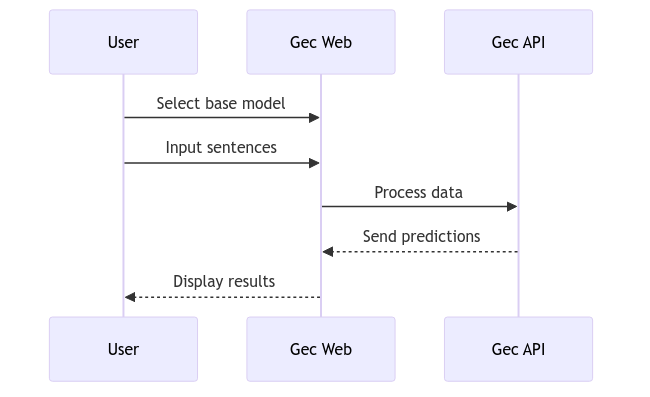
\includegraphics[width=\textwidth]{usecase1}
  \end{center}
  \caption{Sequence Diagram of GecWeb for the main case}\label{fig:usecase1}
\end{figure}

In this use case, user first chooses one of the base models, then input or paste the sentences to be corrected.
Gec Web then pre-process the data and then send it Gec API, where the data is being processes using the selected model.
The corrected sentences is then sent back to Gec Web, where is is being post-process and displayed to the user.

Figure~\ref{fig:usecase2} describes a more advanced use case of GecWeb, where users select multiple models, and the system enables highlighting to indicate the changes made by the correction process.
Since multiple models are used, system combination methods such as ESC or MEMT are applied to improve correction accuracy.

\begin{figure}[htbp]
  \begin{center}
    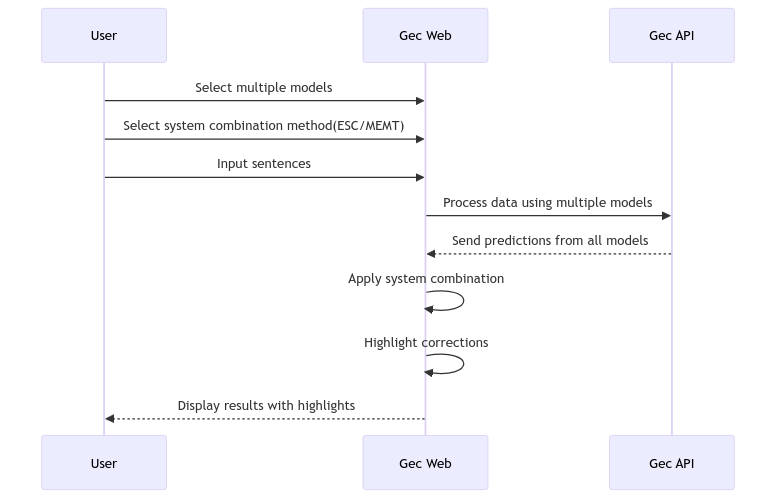
\includegraphics[width=\textwidth]{usecase2}
  \end{center}
  \caption{Sequence Diagram of GecWeb for advanced use case}\label{fig:usecase2}
\end{figure}

In this use case, the user first selects multiple grammatical error correction models (up to 3 models at once).
Then the user selects a system combination method, or leave it default to use ESC.
After inputting or pasting the text to be corrected, GecWeb pre-processes the data and sends it to the Gec API, which runs each selected model separately.
The predictions from all models are then returned to GecWeb, where the selected combination system is applied to merge the outputs and produce a refined correction.

Additionally, the highlight feature is enabled to visualize the modifications.
Changes such as insertions, deletions, and replacements are marked in different colors to provide better clarity on how the text has been corrected.
Finally, the post-processed and highlighted results are displayed to the user.

This approach enhances correction accuracy by leveraging multiple models and improves user experience by making the corrections more transparent.

\section{Non-functional requirement}
\label{non-functional-requirement}

The non-functional requirements for GecWeb focus on ensuring high performance, reliability, usability, maintainability, security, and efficient technical implementation.

In terms of performance, the system should be capable of processing text corrections rapidly, with a target speed of at least 500 words per second when running on a standard GPU server.
This ensures that users experience minimal latency when submitting text for correction, making the application suitable for real-time use.

Reliability is another critical requirement, as GecWeb should maintain high availability with minimal downtime.
The system must incorporate robust error-handling mechanisms to prevent crashes or unexpected failures, ensuring a seamless user experience even under high load conditions.

To enhance usability, the user interface should be designed for intuitive navigation, making it accessible even to users with limited technical expertise.
A clean and responsive design will allow users to focus on their text corrections without unnecessary complexity.

Maintainability is also a key consideration.
The system should follow a modular architecture, making it easy to extend and update.
This modular approach will facilitate the integration of new grammatical error correction models and combination methods without requiring major modifications to the core system.

Security and privacy are paramount, with all API communications secured using HTTPS to protect user data.
Since the system processes text in real-time and does not require data storage, privacy concerns related to user-submitted content are minimized.

From a technical perspective, GecWeb is designed to operate without a database, as all text processing occurs in real-time.
The underlying grammatical error correction models will be hosted on a GPU-powered server to ensure fast inference speeds, supporting high-performance processing while maintaining efficiency.

\section{Conclusion}
\label{conclusion}

In conclusion, this chapter provides a comprehensive analysis of the current state of GEC systems, user needs, and the functional and non-functional requirements for GecWeb.
The next chapter will delve into the methodologies and technologies used to develop the system.
